\chapter{Object Reconstruction at ATLAS}
\label{chap:reconstruction}

%\indent This chapter covers the reconstruction of physics objects at ATLAS.  
\indent The subject of object reconstruction and calibration at ATLAS can easily fill a document that is multiple times the size of the thesis.  The following sections give a brief summary of each object reconstruction algorithm.  Section \ref{sec:reco:IDtrack} covers the reconstruction of inner detector tracks.  Section \ref{sec:reco:vtx} covers the reconstruction of vertices. Section \ref{sec:reco:jets} summarizes the reconstruction and calibration of hadronic jets.  Sections \ref{sec:reco:EM} and \ref{sec:reco:muon} describe the reconstruction and calibration of electrons, photons and muons.  Lastly, section \ref{sec:reco:MET} discusses the reconstruction of missing transverse momentum ($\met$). Greater detail on each subject can be found in the references cited in each section.

\section{Inner Detector Track Reconstruction}
\label{sec:reco:IDtrack}

\indent  Many reconstructed physics objects depend on tracking information in the inner detector (ID).  ID tracks are combined with the EM calorimeter and muon spectrometer information to identify and measure the momentum of electrons and muons.  Hadronic jets use ID tracks to determine if the jet originated from a heavy flavored hadron containing b-quarks or only light flavored hadrons.  ID tracks are also crucial to identifying whether objects originate from the interesting hard scattering interaction or a less interesting pile-up interaction.\\

\indent Two types of inner detector tracks are reconstructed, primary tracks and secondary tracks.  Primary tracks originate from the interaction point (IP) and are meant to reconstruct the trajectories of charged particles originating directly from the proton-proton collisions.  Secondary tracks target charged particles originating in the ID from secondary decays and interactions such as $\gamma \rightarrow e^{+}e^{-}$ conversions.  \\

\indent Primary tracks are reconstructed using the {\tt NEWT} algorithm.  The {\tt NEWT} algorithm starts from seed segments in the inner silicon detectors and extended outwards towards the TRT. Greater details can be found in reference [\cite{NEWT}]. A brief summary of the track reconstruction algorithm will be given here.\\ 

\indent First, seed segments are created from three space point measurements in silicon detectors.  Each pixel cluster corresponds to a single space point measurement since a single pixel sensor provides 3D position information.  Two SCT clusters from the same SCT layer must be combined to form a single space point measurement because each SCT strip only provides 2D position information.  \\

\indent Seed segments can be formed out of all pixel (PPP), all SCT (SSS) or two pixel and one SCT (PPS) space points.  PSS space points are rejected due to high fake rates.  \\

\indent Starting from the original seed segment, track reconstruction is extrapolated layer by layer through the inner detector. Hits are added to the track one layer at a time.  If multiple tracks share a hit, then the shared hit is assigned to the most precise track.  \\%If multiple charged particles are close together when they traverse a pixel layer, they can form merged clusters in the Pixel detector.  These merged pixel clusters are split using a set of trained neural networks. \\

\indent In contrast, secondary tracks are reconstructed from the TRT and extrapolated inwards towards the direction of the beam line.  Segments are reconstructed in the TRT and then extended inwards by adding silicon hits. \\

\section{Vertex Reconstruction}
\label{sec:reco:vtx}

\indent On average around 25 proton-proton interactions occur in every beam crossing in Run 2.  These p-p interactions are spread out in the $Z$ coordinate due to the finite bunch length at the LHC.  We are able to reconstruct the original interaction vertex (primary vertex) by tracing back charged particle tracks to the beam line.  We are able to differentiate objects from the interesting hard scattering p-p interaction from other pileup interactions using reconstructed vertexes.  A summary of the primary vertex reconstruction algorithm is given in this section.  \\

\indent A subset of reconstructed ID tracks are used to reconstruct the primary vertexes.  In Run 2 tracks must satisfy:

\begin{itemize}
\item[] $\pt > 400 \mev$
\item[] $|\eta| < 2.5$
\item[] number of silicon hits $ \ge 9$ if $|\eta| \le 1.65$ or $\ge 11$ if $|\eta| > 1.65$
\item[] IBL hits + B Layer hits $\ge 1$
\item[] maximum $1$ shared module ($1$ shared pixel hit or $2$ shared SCT hit)
\item[] pixel holes $= 0$
\item[] SCT holes $\le 1$
\end{itemize}

\indent A vertex seed is found by searching for the global maximum in the $Z$ coordinate of reconstructed tracks.  The vertex position is fitted using an algorithm that is robust to additional noise and outlier tracks called the adaptive vertex fitting algorithm \cite{VertexReco,adaptiveFitting}.  \\

\indent Adaptive fitting determines the vertex position using a least squared fitting method, but gives the outlier tracks lower weights in the fit.  The vertex position is repeatedly fitted until the fit position no longer changes. A new vertex center is found and new set of weights is calculated for each new fit.  The weighting function also changes from fit to fit according to a predeterminate way; giving more weight to a smaller sub-set of tracks each iteration, ultimately approaching a step function.  \\%The final set of tracks selected is fitted to determine the final position and uncertainty of the vertex. \\

\indent This method of lowering the weight of outlier tracks in each fit and decreasing the weight in each iteration is called determinist annealing. \cite{adaptiveFitting}  The procedure is analogous to repeatedly heating and cooling metal in a forge to make the metal's crystal lattice more regular.  At each iteration, a more compact and regular set of tracks are selected eventually ending in a fix set of selected tracks.  \\

\indent  After determining the vertex position, all tracks within $7\sigma$ of the vertex is considered to be associated with the vertex.  A conservative $7\sigma$ acceptance is used to avoid one energetic vertex being split into two during reconstruction.  Tracks incompatible with the vertex from a new vertex seed.  This process is repeated until all tracks have been clustered into vertexes or no additional vertexes can be found.  Each vertex must have at least two associated tracks. \\

\indent The primary vertex with the highest total $\pt$ summed over all associated tracks is identified as the vertex of the hard scattering interaction.  All other primary vertexes are referred to as pileup vertexes.


\section{Hadronic Jets}
\label{sec:reco:jets}

\indent Energetic partons carrying color charge produced in the initial hard scattering will quickly fragment into multiple hadrons.  The result is a shower of charged and neutral hadrons referred to as a parton shower.  The parton shower leaves a roughly conical energy deposit in the electromagnetic and hadronic calorimeter and multiple associated tracks in the inner tracker.  Some energy may even be deposited in the muon spectrometer if the initial hadron is energetic enough.  This detector signature is referred to as a jet. \\

\indent Identification and reconstruction of hadronic jets is very important for many different detector signatures including this analysis.  Of key importance is the correct reconstruction of the initial parton energy.  Also important is the rejection of jets resulting from pile-up interactions and identifying jets resulting from b-quarks.  Jet reconstruction and energy calibration are described in sections \ref{sec:jet:reco} and \ref{sec:jet:calib}.  Jet vertex tagging and b-jet tagging are described in section \ref{sec:jet:JVT} and \ref{sec:jet:btag}.

\subsection{Hadronic Jet Reconstruction}
\label{sec:jet:reco}

\indent Hadronic jets are reconstructed by clustering energy deposits in the calorimeter. First, all topologically connected calorimeter cells are clustered around a seed cell that passes the $4\sigma$ signal above noise threshold.  These 3D clusters are referred to as topological clusters (topo-clusters).\cite{jetReco7TeV,jetReco13TeV}  Neighboring cells around the cluster are added to the cluster if they pass a $2\sigma$ signal over noise threshold. This step is repeated until no neighboring cells pass the $2\sigma$ signal over noise threshold.  At this stage, one last round of neighboring cells is added regardless of the amount of signal to noise ratio in those cells. \\

\indent Topo-clusters are then grouped into jets according to the $\antikt$ algorithm.  The $\antikt$ algorithm groups objects according to the distance measure $d_{ij}$ defined in equation \ref{eqn:antikt} with parameter $p=-1$.  All objects within $d_{ij}$ less then $d_{iB}=k^{2p}_{Ti}$ are grouped into a single jet.  \\

\begin{equation}
d_{ij} = min ( k^{2p}_{Ti}, k^{2p}_{Tj} ) \frac{(\Delta\eta^2_{ij} + \Delta\phi^2_{ij})}{R^2}
\label{eqn:PileupDensity}
\end{equation}

\indent  The algorithm can best be explained by examining an example case.  If a hard object $1$ exists and is surrounded by only soft objects $j$ then $d_{1j}$ equals $k^{2p}_{1j}(\frac{\Delta R^2}{R^2})$ for all $j$ where $\Delta R = \Delta \eta^2 + \Delta \phi^2$.  $d_{1j}$ will always be less then any $d_{ij}$ if both $i$ and $j$ are both soft and have the same $\Delta R$ as $1$ and $j$.  Therefore, the $\antikt$ algorithm effectively groups hard objects first before soft objects.  \\

\indent A perfectly conical jet of radius $R$ will be formed if no other hard objects are found within a cone of $2R$.  If two hard objects exist within $R<\Delta R_{1,2}<2R$ of one another then two jets will be formed splitting the energy cells between them.  If two hard objects exist within $\Delta R_{1,2}<R$ then they will both be grouped into a single jet. \\

\indent  The $\antikt$ algorithm is both infrared and collinear safe.  Meaning the algorithm is insensitive to the radiation of additional soft particles and the collinear splitting of initial partons.  Additional soft partons do not change the shape of the jets but the jet shape is flexible to accommodate the presence of other hard radiation. \\

\indent ID Tracks are associated with jets according to a ghost association procedure.\cite{JetAreaGhostAssociate}  Tracks with the same direction and location as real ID tracks but infinitesimally low $\pt$ are allowed to be clustered by the $\antikt$ algorithm.  If these tracks are assigned to the jet by the $\antikt$ algorithm then the real track is associated with the jet.  In this way, we can determine which tracks are associated with the jet without disturbing the clustering of calorimeter energy.  The same procedure of clustering infinitesimally low $\pt$ objects is used to determine the jet area. \\

\subsection{Jet Calibration and Systematics}
\label{sec:jet:calib}

\indent Both the electromagnetic and hadronic calorimeters at ATLAS are sampling calorimeters.  The energy deposited in the absorber material is effectively lost because the absorber do not actively record a signal.  Therefore the energy measured using the active material must be scaled up to compensate for this loss.  For this reason and others including leakage of energy outside of the calorimeter edges and deposition of energy below the energy thresholds, reconstructed jets must be calibrated to determine the original hadron's energy.  \\

\indent  A variety of MC based and data based methods are used to calibrate hadronic jets.  Figure \ref{fig:jetCalibFlow} shows the steps in jet calibration for Run 2.\cite{Calibartion13TeV} \\

\begin{figure}[htb]
  \begin{center}
    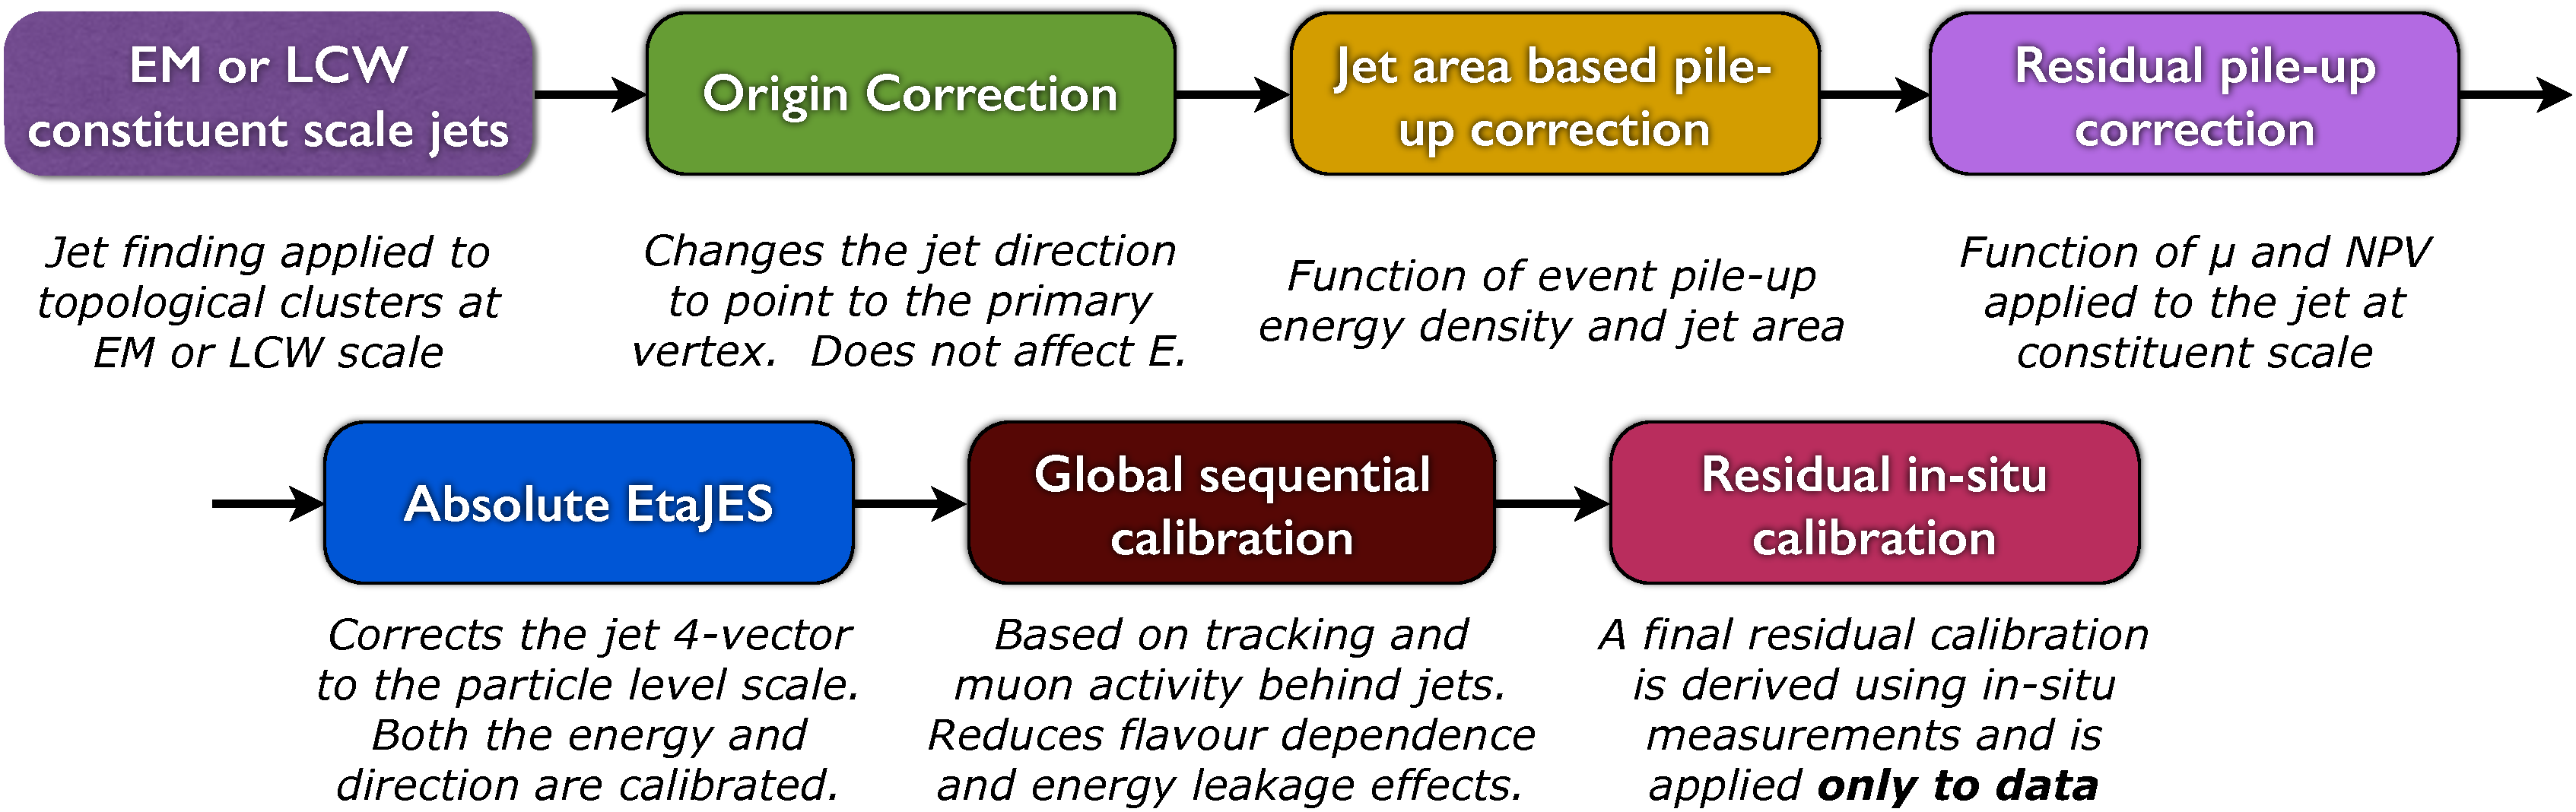
\includegraphics[width=0.85\textwidth]{figures/JetCalib/JetCalibFlow.png}\hspace{0.05\textwidth}
\end{center}
\caption{Flow chart of the steps involved in jet calibration. (Figure taken from \cite{Calibartion13TeV}) }
\label{fig:jetCalibFlow} 
\end{figure}

\indent First the individual topo-clusters in the jet are calibrated to the energy scale of EM showers using MC simulations.\cite{topoCalib}  It should be noted that this calibration is to EM showers correctly calibrates the energy in EM showers but underestimates the amount of energy lost in hadronic showers.  Additional corrections are applied in the following steps to account for this difference. \\
% The origin of the reconstructed jet is also set to the primary vertex instead of the default detector center. \\

\indent A correction for energy deposited by pileup interactions are applied.\cite{pileupsub}  The correction is based on the measurement of average energy originating from pileup $\rho$ multiplied by the measured jet area.  The pileup energy density is defined in equation \ref{eqn:PileupDensity} and determined by measuring the median energy density of $R=0.4$ $k_t$ jets found in the central $|\eta|<2.0$ part of the calorimeter.  The $k_t$ algorithm preferentially cluster soft objects first instead of hard objects and is more sensitive to soft pileup radiation and no $\pt$ thresholds are applied to the reconstructed $k_t$ jets as we are trying to measure soft objects.  \\

\begin{equation}
\rho=median\{ \frac{p_{T i}^{k_t~jet}}{A_i^{k_t~jet}} \}
\label{eqn:PileupDensity}
\end{equation}

\indent The area based pileup energy correction is subtracted along with two other residual corrections.  The total pileup correction to jet $\pt$ is given in equation \ref{pilupCorrection}. \\

\begin{equation}
p_T^{corr} = p_T - \rho \times A - \alpha~\times (N_{PV} - 1 ) - \beta~\times <\mu>
\label{eqn:pilupCorrection}
\end{equation}

\indent  It should be noted that the jet energy response still has a dependence on pileup after this area based correction has been applied.  The sources of this dependence can be attributed to the incomplete cancelation of in-time and out-of-time pileup.\cite{JetCalibartion13TeV}  For example, events with a low number of reconstructed vertexes ($N_{PV}$) in a run with high average number of interactions per bunch crossing ($<\mu>$) may receive relatively large amounts of out-of-time pileup compared to in-time pileup.  This effect is also parameterized by using the constants $\alpha$ and $\beta$ in equation \ref{pilupCorrection}. \\  

\indent In the next step, the jet energy scale (JES) is applied.  JES is a scale factor which relates the reconstructed jet energy with the true jet energy.  JES is calibrated using a number of MC and data driven methods.  The JES is derived from an inclusive jet MC after pileup and origin corrections have been applied.  \\

\indent A residual difference between the energy responses of gluon and light quark jets remains after JES calibration.\cite{JetCalibartion13TeV}  The difference can be as large as 8 percent and is due to a number of reasons including the factor of 2 difference in color charge between quarks and gluons.  A global sequential correction scheme (GSC) is applied to account for this deference and correct for other detector based issues.\cite{jet_GSC}  \\

\indent GSC corrections uses information on the topology of energy deposits, associated inner detector tracks and activity in the muon spectrometer behind the jet.  ID Tracking information is used to reduce the flavour dependence because gluon initiated jets tend to have a wider profile and more tracks. Muon spectrometer information is used to better estimate high energy jets which penetrate the full depth of the calorimeter.  Information on the relative amount of calorimeter energy deposited in specific layers is used to improve the jet energy resolution. \\

\indent Lastly, further corrections to the jet energy response are obtained by measuring the balance between jets and some reference objects directly in data. \cite{JES_ZGamma,JES_dijet}  The reference object can be a photon, a $Z$ boson or other jets.  The $\pt$ balance between jets and the reference objects are measured in data and compared to the MC.  A residual correction is applied by the data over MC ratio based on equation \ref{jet_insitu}.  Systematic uncertainties on the jet energy responses including those on the jet energy scale and jet energy resolution are also derived using these data driven methods. \\

\begin{equation}
\frac{R_{data}}{R_{MC}} = \frac{<p_T^{jet}/p_T^{ref}>_{data}}{<p_T^{jet}/p_T^{ref}>_{MC}}
\label{eqn:jet_insitu}
\end{equation}

\indent The jet $\pt$ resolution for $|\eta|<0.8$ and $0.8<|\eta|<1.2$ jets are shown in figure \ref{fig:jet_ptresolution}.\cite{JES_dijet} \\

\begin{figure}[htb]
  \begin{center}
    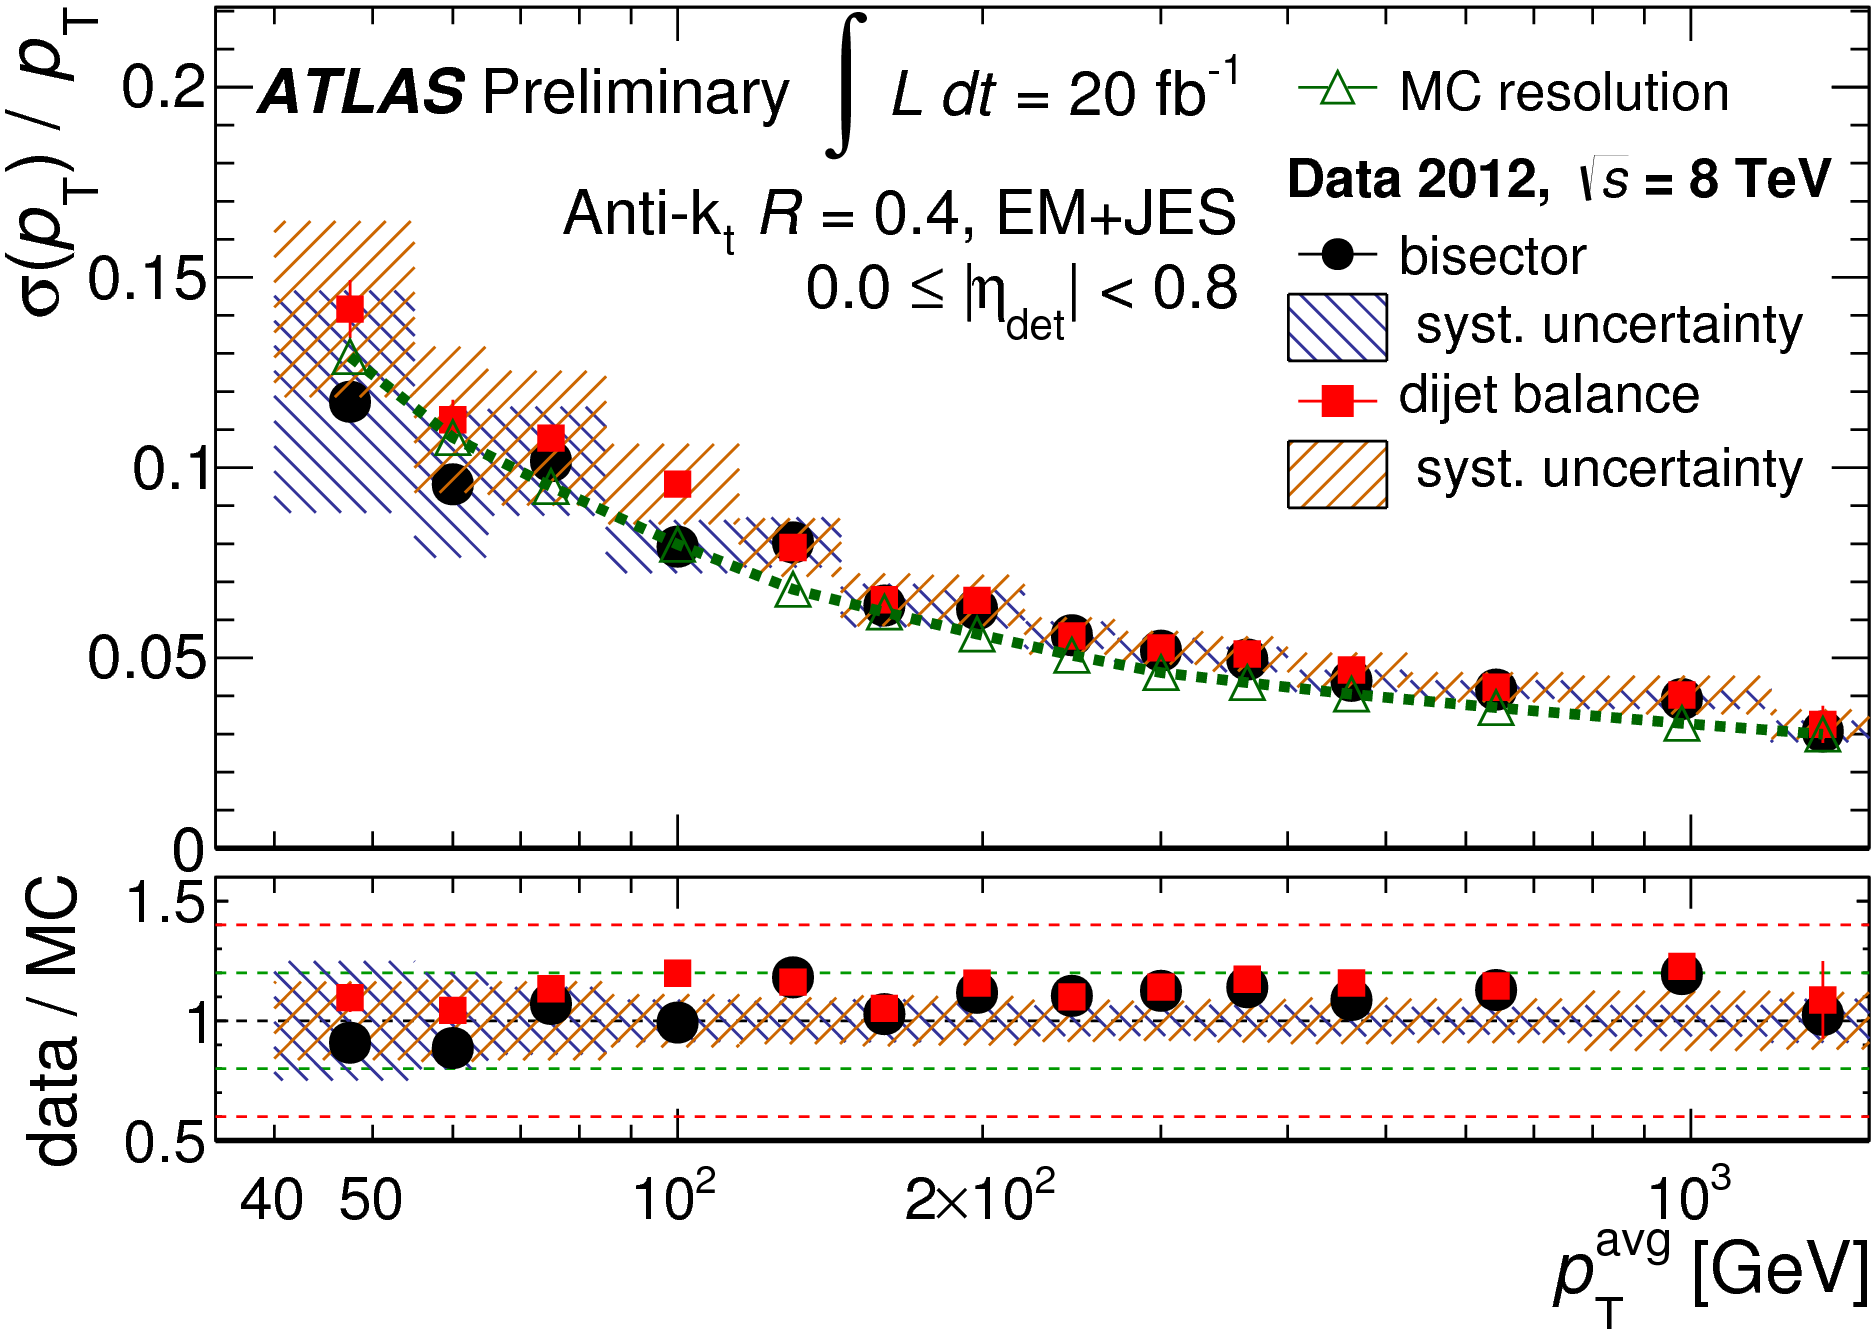
\includegraphics[width=0.45\textwidth]{figures/JetCalib/JetCentral_Response.png}\hspace{0.05\textwidth}
    \includegraphics[width=0.45\textwidth]{figures/JetCalib/JetTransition_Response.png}\hspace{0.05\textwidth}
\end{center}
\caption{Jet $\pt$ resolution for $|\eta|<0.8$ and $0.8<|\eta|<1.2$ jets as a function of jet $\pt$ in 8 TeV data. (Figure taken from \cite{JES_dijet}) }
\label{fig:jet_ptresolution} 
\end{figure}

\subsection{Pileup Jet Rejection and Jet Vertex Tagger}
\label{sec:jet:JVT}

\indent It is imperative to be able to distinguish between jets originating from the hard scattering interaction (hard scattering jets) and those originating from other pile-up interactions (pileup jets) in the high luminosity LHC environment.  Pileup jets may originate from both the on average 25 additional p-p interactions in the same bunch crossing or from interactions in other beam crossings.  We distinguish between the hard scattering jets from pileup jets using a multivariate discriminate known as the jet vertex tagger (JVT).\cite{JVT} \\

\indent The JVT discriminate is based on two variables $\corrJVF$ and $\RpT$ defined in equations \ref{eqn:corrJVF} and \ref{eqn:RpT}.

\begin{equation}
\corrJVF = \frac{\sum_i p_T^{trk_i} (PV_0) }{ \sum_l p_T^{trk_l} (PV_0) + \frac{\sum_{n\ge1} \sum_l p_T^{trk_l} (PV_n) }{k\dot n^{PU}_{trk}} }
\label{eqn:JVF}
\end{equation}

\begin{equation}
\RpT = \frac{\sum_i p_T^{trk_i} (PV_0) }{ p_T^{jet} }
\label{eqn:RpT}
\end{equation}

\indent The $\corrJVF$ variable roughly corresponds to the fraction of a jet's ID track $\pt$ that originate from the hard scattering vertex.  $\sum_i p_T^{trk_i} (PV_0)$ is the sum of all jet's associated track $\pt$ that originate from the primary vertex $PV_0$.  The quantity $p^{PU}_T = \sum_{n\ge1} \sum_l p_T^{trk_l} (PV_n)$ is the total amount of a jet's associated track $\pt$ that originates from pile up interactions.  $p^{PU}_T$ is divided by $k\dot n^{PU}_{trk}$ to correct for the fact that $<k\dot n^{PU}_{trk}>$ will increase linearly with the number of pileup vertexes $n^{PU}_{trk}$.  This makes the variable $\corrJVF$ roughly independent to the number of reconstructed vertexes. The value $k$ is set to an arbitrary $0.01$ and the discriminating power of JVT was found to be independent of the choice of $k$.\\

\indent $\RpT$ is defined as the total track $\pt$ of all associated tracks that originate from the primary vertex $PV_0$ divided by the fully calibrated jet $\pt$. It is important to note that the calibrated jet $\pT$ includes pileup subtraction.  $\RpT$ peaks sharply at zero for pileup jets.  On the other hand, $\RpT$ corresponds to roughly the charged $\pt$ fraction in hard scattering jets.  \\

\indent The JVT discriminate constructs a 2D likelihood based on these variables.   The JVT discriminate determines the probability that a jet will be a hard scattering jet using the k-nearest neighbor (kNN) multivariate technique \cite{TMVA} trained on a $20<\pt<50 \gev$ and $|\eta|<2.4$ MC sample of hard scattering and pileup jets.  The k-nearest neighbor (kNN) algorithm is robust relative to local fluctuations in sparsely populated regions.  \\

\indent For our analysis we require a jet vertex tagger value greater than 0.59.  This corresponds to a 92 percent efficiency for jets originating from the hard scattering interaction and a 2 percent fake rate from pileup jets, if the jet has $|\eta| < 2.4$ and $\pt < 60 \gev$.  The JVT efficiency as a function of jet $\pt$ is shown in figure \ref{fig:JVT_eff} \\

\begin{figure}[htb]
  \begin{center}
    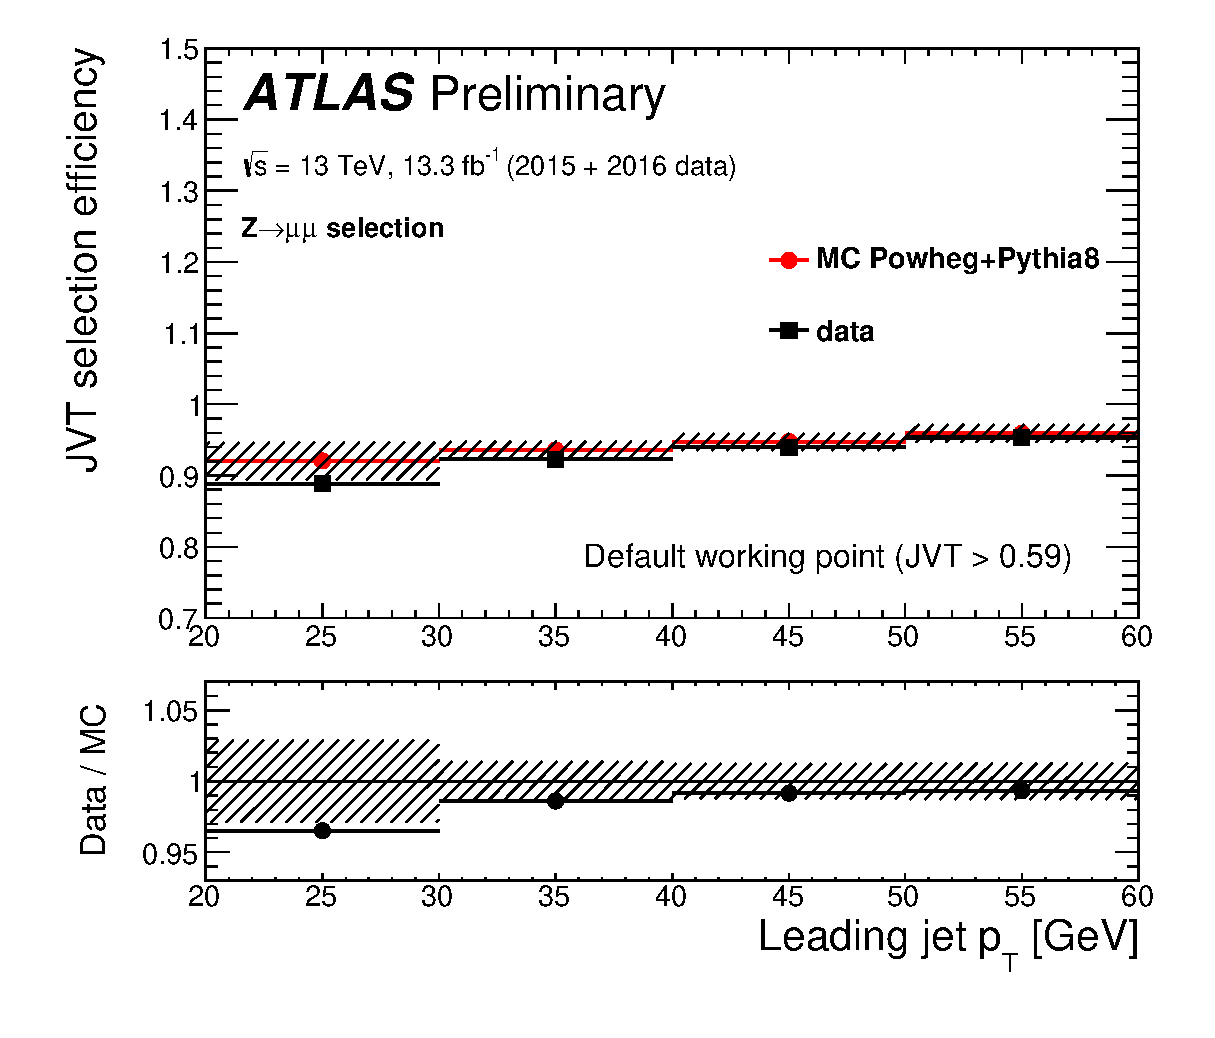
\includegraphics[width=0.65\textwidth]{figures/JetCalib/JVT_eff.eps}\hspace{0.05\textwidth}
\end{center}
\caption{The distribution showing the jet vertex tagger efficiency as a function of jet $\pt$ in 2015+2016 data. Only jets balanced against a $Z->\mu\mu$ boson are accepted.  Details can be found in \cite{JVT}. }
\label{fig:JVT_eff} 
\end{figure}

\subsection{Jet Quality and Jet Cleaning}
\label{sec:jet:quality}

\indent Several variables are useful in discriminating between real hadronic jets and fake jets not coming from p-p interactions.  The sources of fake jets include noise in the LAr and Tile calorimeters, beam induced backgrounds and cosmic raw showers.  These variables can be divided into three broad categories: variables quantifying the EM and hadronic calorimeter energy ratio, ID track based variables and variables based on the pulse shape of the LAr calorimeters.  Detailed descriptions of the variables used can be found in \cite{JetCleaning} a brief summary will be given here.\\

\indent Energy ratio variables can reject calorimeter noise and beam induced backgrounds and energy deposited from cosmic rays.  Jets originating from beam induced backgrounds tend to concentrate more energy in a few longitudinal layers compared to jets from p-p collisions.  Multiple variables corresponding to the fraction of jets energy deposition in any one section along the expected direction of the shower relative to the total energy deposition are useful in discriminating against fake jets. \\

\indent Energy ratio variables include: \\

\begin{itemize}
\item[] $f_{EM}$: ratio of EM calorimeter energy to total jet energy
\item[] $f_{HEC}$: ratio of HEC calorimeter energy to total jet energy
\item[] $f_{max}$: maximum energy fraction in any single calorimeter layer
\end{itemize}

\indent ID track based variables are useful because tracks can be matched to the primary vertexes in good jets.  Fake jets have low fraction of tracks which can be matched to primary vertexes.  \\

\indent list of track based variables include: \\

\begin{itemize}
\item[] $f_{ch}$: ratio of the scalar sum of ID track $\pt$ where ID track must originate from the primary vertex to jet $\pt$.  approximately the fraction of jet energy carried by charged particles.  
\item[] $f_{ch}/f_{max}$: ratio of $f_{ch}$ and $f_{max}$, the maximum energy fraction in any single calorimeter layer
\end{itemize}

\indent Pulse shape in the LAr should be consistent with those of a particle shower in good jets.  A quality variable $Q^{LAr}_{cell}$ measures the quadratic difference between expected and actual pulse shapes in each LAr cell.  Quality variables based on the fraction of cells in a jet with poor quality and the average quality is found to provide discrimination power against LAr noise. \\

\indent LAr pulse shape variables include: \\

\begin{itemize}
\item[] $\braket{Q}$: weighted average of pulse quality of LAr cells ($Q^{LAr}_{cell}$) in a jet.  Normalized to $0 < \braket{Q} < 1$.
\item[] $f^{LAr}_{Q}$: Fraction of energy in cells with poor quality pulse shapes in EM LAr Calorimeter
\item[] $f^{HEC}_{Q}$: Fraction of energy in cells with poor quality pulse shapes in hadronic endcap calorimeters (HEC) which also use LAr technology.
\item[] $E_{neg}$: total energy of all cells with negative energy
\end{itemize}

\indent A jet satisfying any one of the following criteria is considered a {\tt BadLoose} jet.  The presence of a {\tt BadLoose} can result in poor $\met$ reconstruction due to a noisy calorimeter or beam induced background.  Therefore, if any baseline jet in the event is found to be {\tt BadLoose} then the entire event is rejected.   This procedure is called jet cleaning.  \\

\indent A jet is considered a {\tt Loose} jet if is not identified as a {\tt BadLoose} jet.  {\tt Loose} jets are used as signal jets in most ATLAS physics analysis including this one. \\

\begin{enumerate}
\item[] $f_{EM} > 0.5$ and $|f^{HEC}_{Q}| > 0.5$ and $\braket{Q} > 0.8$
\item[] $E_{neg} > 60 \gev$
\item[] $f_{EM} > 0.95$ and $f^{LAr}_{Q} > 0.8$ and $\braket{Q}>0.8$ and $|\eta|<2.8$
\item[] $f_{max}>0.99$ and $|\eta|<2.0$
\item[] $f_{EM}<0.05$ and $f_{ch}<0.05$ and $|\eta|<2$
\item[] $f_{EM}<0.05$ and $|\eta|\ge2$
\end{enumerate}

\subsection{Identifying Jets Originating from Heavy Flavor Hadrons}
\label{sec:jet:btagging}

\indent Hadrons containing b-quarks have long lifetimes, around 1.5 ps or a $c\tau$ of roughly 450 $\mu$m.  The long flight distance allows us to reconstruct ID tracks with large impact parameters and perhaps reconstruct secondary vertexes. \\% The typical b-hadron decay consist of at least one vertex displaced from the point of initial hard scattering.  \\

\indent Three separate algorithms have been setup to distinguish jets originating from b-hadrons (b-jets) from light hadrons and c-hadrons (c-jets).  A brief description of each algorithm is given in this section.  More details can be found in \cite{btagging2016}  and \cite{btagging2015}.  \\

\indent The first algorithm is based on track impact parameters for high quality tracks that are associated with jets.  The discriminate is computed as a sum of the log likelihood ratio of each accepted track in the vertex or $\sum_i \ln(\frac{p_b}{p_{light}})$, where i sums over all accepted tracks in the jet and $p_b$ is the PDF for a b-jet and $p_{light}$ is the PDF for a light jet.  The PDF uses transverse and longitudinal impact parameters $d_0$ and $z_0$ as observables and is derived from MC simulation.  \\

\indent The second algorithm seeks to reconstruct the secondary vertex associated with the b-hadron decay.  This algorithm has the advantage that if a secondary vertex is consistent with the decays of long lived hadrons that do not contain b-jets such as $K_s$ or $\Lambda$ or photon conversions then the vertex maybe rejected.  For example, secondary vertexes with a mass greater then $6 \gev$ are inconsistent with b decays and are rejected. Variables based on the secondary vertex location, energy, and mass can all be used to discriminate b-jets from light-jets and c-jets.  \\

\indent The third algorithm attempt to reconstruct the full b-hadron decay chain and is called the decay chain multi-vertex reconstruction algorithm.  The algorithm uses a Kalman filter to determine the common line on which the primary vertex and the bottom/charm vertexes lie.  \\

\indent The output of the three algorithms are all combined into a multivariate discriminate called MV2.  MV2 uses a boosted decision tree (BDT) algorithm \cite{TMVA} to gain better separation power between different jet flavors. This analysis uses the MV20c10 discriminate to tag b-jets. MV20c10 is selected as it gives the best balance between light jets and c-jet rejection for a given b-tagging efficiency.  \\

\indent The b-tagging efficiencies and mis-tag rates have been calibrated by the ATLAS flavor tagging group.  The distribution of the MV20c10 discriminate for light, charm and b-hadrons can be seen in figure \ref{fig:MV20c10}. We make a selection at MV2c10 $ > 0.6459$ which corresponds to approximately 77\% b-tagging efficiency with a factor of 134 reject rate for light jets.  \\

\begin{figure}[htb]
  \begin{center}
    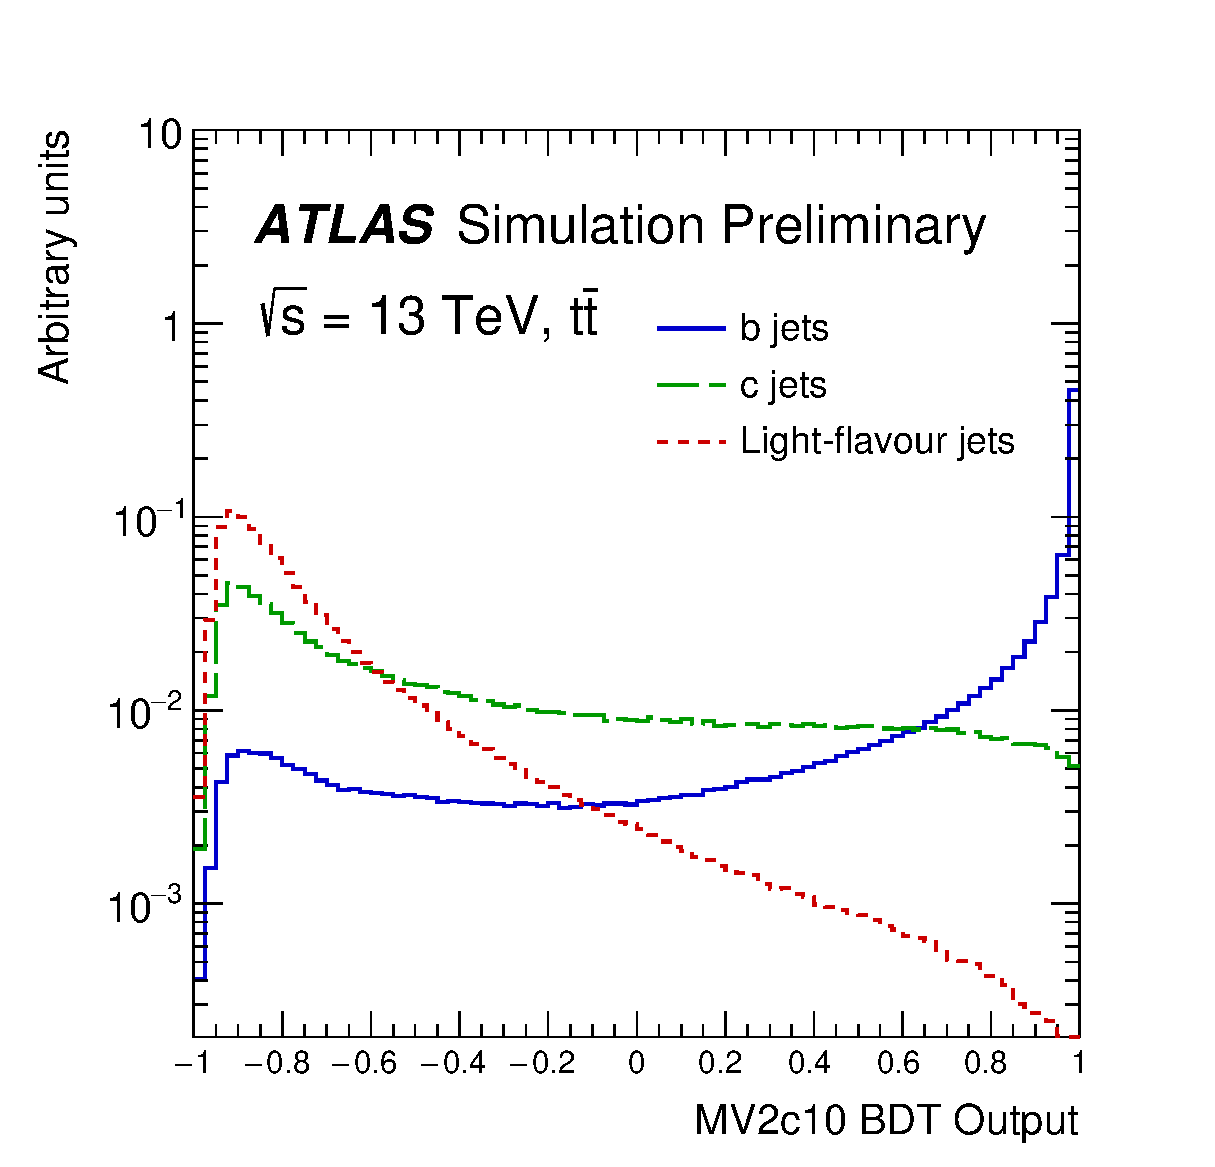
\includegraphics[width=0.85\textwidth]{figures/JetCalib/MV20c10.eps}\hspace{0.05\textwidth}
\end{center}
\caption{Distribution of the MV20c10 multivariate discriminate used for tagging b-jets.  Figure taken from \cite{btagging2016}  }
\label{fig:MV20c10} 
\end{figure}


\section{Electron and Photons}
\label{sec:reco:EM}

\subsection{Electron and Photon Reconstruction}
\label{sec:reco:EM}

\indent Both electron and photon reconstruct starts from clusters of energy deposits in the electromagnetic calorimeter.  The EM calorimeter is first divided into a grid of towers each with the size of $\Delta \eta \times \Delta \phi = 0.025 \times 0.025$.  The energy of all cells in the longitudinal layers inside each tower is summed into the total tower energy.  \\

\indent The EM clusters are seeded by towers with energy above a certain threshold.  A sliding-window algorithm then groups the energy towers near the seed into EM clusters.\cite{EMReco13TeV,EMReco8TeV}  The window width is $3 \times 7$ towers in the barrel and $5 \times 5$ towers in the endcap.  The reconstructed cluster therefore has a size of $\Delta \eta \times \Delta \phi = 0.075 \times 0.175$ in the barrel and $ 0.125 \times 0.125$ in the endcap.  The same window size is used for electrons and photons to ensure better cancelation of systematics when using electrons to measure photon response.\cite{EMReco13TeV}  The window position is adjusted so that the reconstructed cluster energy is the local maximum.  The different cluster sizes were optimized for the different energy distribution in the barrel and endcap calorimeters while minimizing pileup and noise contributions.\cite{EMReco13TeV}  \\

\indent Identified clusters are then matched to reconstructed ID track using track and cluster position.  ID tracks are required to have a minimum number of pixel and total silicon hits.  Clusters are considered an electron candidate if a single well-reconstructed ID track that originates from a vertex is found.  The cluster is considered an unconverted photon candidate if no tracks are found.  The cluster is considered a converted photon candidates if two opposite signed tracks that are collinear, originate from the interaction point, and are consistent with electrons are present.  The cluster if also considered a converted photon if a single track is present but the track lacks hits in the IBL of the pixel detector.  \\

\indent Furthermore, electron and photon candidates must satisfy a set of criteria.  These variables include descriptions of the EM shower shapes, amount of hadronic activity behind the EM calorimeter and properties of associated tracks.  More details on electron and photon identification are given in section \ref{sec:reco:eleQuality} and \ref{sec:reco:phoQuality}. \\

\subsection{Electron Identification and Quality}
\label{sec:reco:eleQuality}

\indent Electron identification in Run 2 is based on a likelihood algorithm that depends on a list of kinematics variables including EM shower shape, EM vs hadronic activity ratio, activity in the TRT and properties of the associated track.  The list of variables included in the likelihood can be found in \cite{EleID}.  A multivariate technique is used to ensure the PDF estimation is robust in low statistics regions in the high dimensional space.  Probability density functions (PDF) are formed for electrons and non-electron backgrounds for a set of discriminating variables used on MC.  The probability of the candidate being an electron is calculated using the two PDFs.  \\

%TypeDescriptionNameHadronic leakageRatio ofETin the first layer of the hadronic calorimeter toETof the EM clusterRhad1(used over the range|?|<0.8 or|?|>1.37)Ratio ofETin the hadronic calorimeter toETof the EM clusterRhad(used over the range 0.8<|?|<1.37)Back layer ofRatio of the energy in the back layer to the total energy in the EM accordionf3EM calorimetercalorimeter. This variable is only used below 100 GeV because it is known tobe inefficient at high energies.Middle layer ofLateral shower width,q(?Ei?2i)/(?Ei)?((?Ei?i)/(?Ei))2, whereEiis thew?2EM calorimeterenergy and?iis the pseudorapidity of celliand the sum is calculated withina window of 3�5 cellsRatio of the energy in 3�3 cells over the energy in 3�7 cells centered at theR?electron cluster positionRatio of the energy in 3�7 cells over the energy in 7�7 cells centered at theR?electron cluster positionStrip layer ofShower width,p(?Ei(i?imax)2)/(?Ei), whereiruns over all strips in a windowwstotEM calorimeterof??�???0.0625�0.2, corresponding typically to 20 strips in?, andimaxis the index of the highest-energy stripRatio of the energy difference between the largest and second largest energyEratiodeposits in the cluster over the sum of these energiesRatio of the energy in the strip layer to the total energy in the EM accordionf1calorimeterTrack conditionsNumber of hits in the innermost pixel layer; discriminates againstnBlayerphoton conversionsNumber of hits in the pixel detectornPixelNumber of total hits in the pixel and SCT detectorsnSiTransverse impact parameter with respect to the beam-lined0Significance of transverse impact parameter defined as the ratio ofd0d0/?d0and its uncertaintyMomentum lost by the track between the perigee and the last?p/pmeasurement point divided by the original momentumTRTLikelihood probability based on transition radiation in the TRTeProbabilityHTTrack-cluster??between the cluster position in the strip layer and the extrapolated track??1matching??between the cluster position in the middle layer and the track extrapolated??2from the perigeeDefined as??2, but the track momentum is rescaled to the cluster energy??resbefore extrapolating the track from the perigee to the middle layer of the calorimeterRatio of the cluster energy to the track momentumE/p6

\indent Electron identification is split into categories {\it very loose, loose, medium, } and {\it tight}.  Each operating point is a sub-set of another.  For example, all tight electrons are also medium electrons and so on.  25 GeV tight electrons have an efficiency of 78 percent and fake rate of 0.3 percent.  25 GeV loose electrons have an efficiency of 90 percent and fake rate of 0.8.  The efficiency increases with $E_T$ while the fake rate decreases.\cite{EleID} \\

\indent Because some shower shape distributions tend to broaden with the number of pileup collisions, the cut on the likelihood discriminant is loosened as a function of the number of vertices. This is done to preserve the identification efficient at high pileup and does not drastically increase the amount of background.\cite{EleID} 

\subsection{Photon Identification and Quality}
\label{sec:reco:photoID}

\indent Photon identification is based on the shower shape and the amount of hadronic activity behind the EM cluster.  The energy deposited in the cells in the first and second layer of the EM calorimeter are important for distinguishing the EM shower originating from photons and those originating the neutral mesons such as $\pi_0$. A detailed list of the discriminating variables used can be found in \cite{photonID}. \\

\indent The requirements are different for converted and unconverted photon candidates to account for the different expected shower shapes.  The requirements are differ in pseudorapidity intervals to account for the varying amount of material upstream of the calorimeter. The requirements were optimized using a multivariate technique.\cite{TMVA}\\

\indent Two working points are included a loose and a tight selection.  The loose ID exploits the variables only in the EM calorimeter and in the hadronic calorimeter layer and is typically used for the trigger and for background studies.  The tight ID uses the full granularity of the EM calorimeter, including the fine segmentation of the first sampling layer, and tightens requirements on the variables used in the loose selection.  The tight working point is the one generally recommended for physics analysis and photons used in this analysis are tight photons.  \\

%CategoryDescriptionNameloosetightAcceptance|?|<2.37, with 1.37<|?|<1.52 excluded??   ?Hadronic leakageRatio ofETin the first sampling layer of the hadroniccalorimeter  toETof  the  EM  cluster  (used  over  therange|?|<0.8 or|?|>1.37)Rhad1?   ?Ratio ofETin the hadronic calorimeter toETof theEM cluster (used over the range 0.8<|?|<1.37)Rhad?   ?EM Middle layerRatio of 3�7?�?to 7�7 cell energiesR??   ?Lateral width of the showerw?2?   ?Ratio of 3�3?�?to 3�7 cell energiesR??EM Strip layerShower width calculated from three strips around thestrip with maximum energy depositws3?Total lateral shower widthwstot?Energy outside the core of the three central strips butwithin seven strips divided by energy within the threecentral stripsFside?Difference  between  the  energy  associated  with  thesecond maximum in the strip layer and the energy re-constructed in the strip with the minimum value foundbetween the first and second maxima?E?Ratio  of  the  energy  difference  associated  with  thelargest and second largest energy deposits to the sumof these energiesEratio?Table 2: Discriminating variables used forlooseandtightphoton identification.20


\subsection{Electron and Photon Energy Calibration}
\label{sec:reco:EMCalibration}

\indent Electron and photon energy must also be calibrated because of the non-compensating nature of the EM calorimeter.  At the same time, the correctly estimating the amount of material upstream of the calorimeter is also important.  Typically a $100 \gev$ electron will deposit between a few percent to 20 percent of its energy before it reaches the calorimeter.\cite{EMReco13TeV} Also about 5 percent of the electron energy may be deposited outside of the cluster.  Electron and photon calibration accounts for all these affects to get an estimate of the true electron and photon energy.  The calibration procedure follow the steps indicated in figure \ref{fig:EMCalibFlow}.

\begin{figure}[htb]
  \begin{center}
    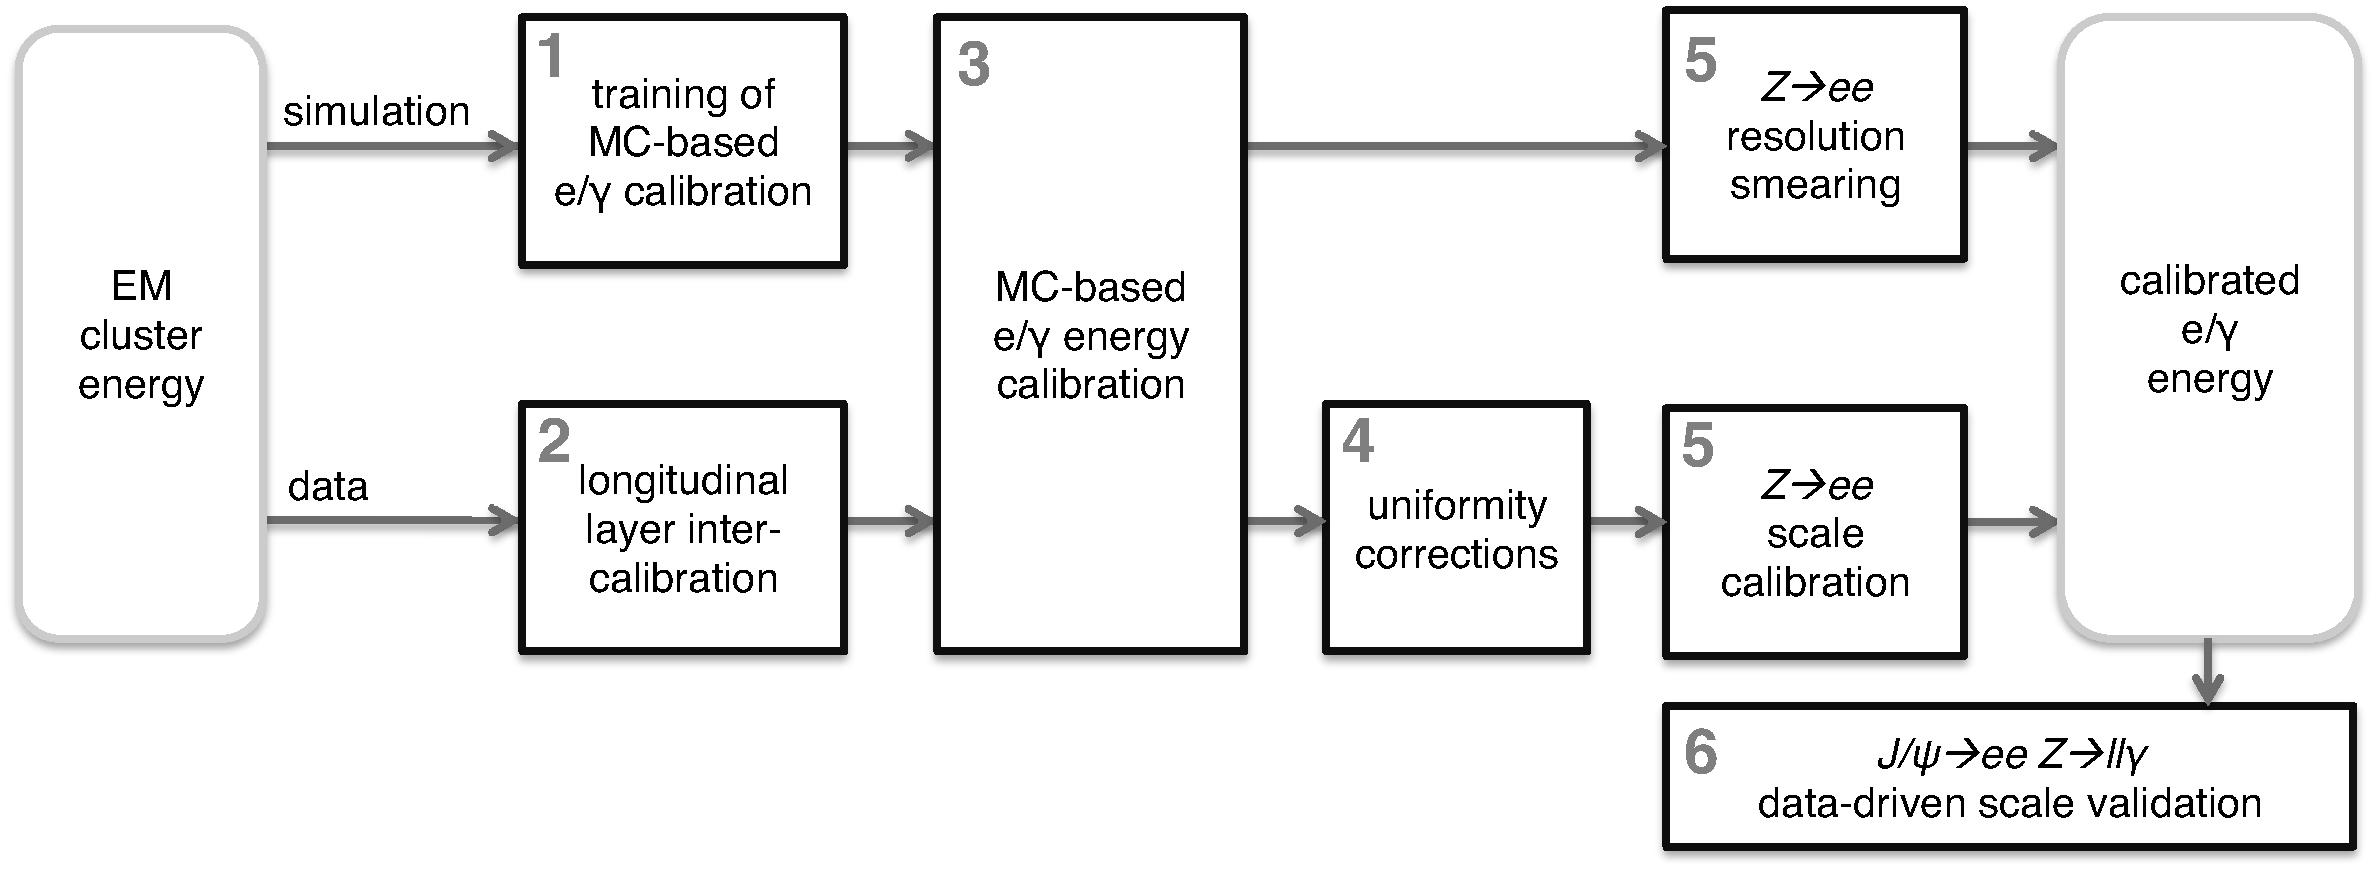
\includegraphics[width=0.85\textwidth]{figures/EMCalib/ElecCalib.png}\hspace{0.05\textwidth}
\end{center}
\caption{Flow chart of the steps involved in the calibration of the energy response of electrons and photons \cite{EMReco8TeV}}
\label{fig:EMCalibFlow} 
\end{figure}

\indent The EM clusters are first calibrated to the original electron or photon energy using a multivariate technique \cite{TMVA} based on MC simulations.\cite{EMReco13TeV,EMReco8TeV}   The MC based calibration uses information on the EM cluster properties such as the longitudinal shower shape and information from any associated ID track.  The response is different for electrons, converted photons and unconverted photons.  \\

\indent The longitudinal layers of the EM calorimeter must be calibrated relative to one another.  Specifically, the relative energy response of the presampler and the first and second layer must be validated by using data.  These cannot be done at the cluster level as clusters sum over all longitudinal layers.  The intercalibration of the first and second layers of the EM calorimeter is performed with $Z\rightarrow\mu\mu$ decays.   This is because the muon energy deposit in the calorimeter are relatively insensitive to the amount of material upstream of the EM calorimeter  The presampler energy scale is calibrated using W and Z decays.  The ratio of data to MC in the presampler energy detected in electrons from W and Z to electron decays is used as a scale factor.  This accounts for mismodeling of the amount of material in front of the presampler. \\

\indent A number of corrections are then applied to account for differences between simulation and data such as regions with non-optimal HV and geometrical affects.  Finally a correction is applied to ensure that the $Z\rightarrow ee$ modeling in simulation agrees with data.  The same scale factors derived for electrons from $Z\rightarrow ee$ is applied to photons but additional photon-specific systematic uncertainties are also applied.  \\

\indent Cross-checks of the electron and photon calibration is performed with $J/\psi \rightarrow ee$ and $Z \rightarrow ll\gamma$ events in data after all energy corrections are applied.  

\section{Muons}
\label{sec:reco:muon}

\subsection{Muon Inner Detector and Muon Spectrometer Track Reconstruction}
\label{sec:reco:IDMStrk}

\indent Muons are first reconstructed independently in the inner detector (ID) and muon spectrometer (MS). Later information from the ID, MS and calorimeter are combined form different types of reconstructed muons.  The type of reconstructed muon depend on the type of information available to be combined.\cite{MuonReco} \\

\indent Muon tracks in the ID are reconstructed using the same algorithm for reconstructing all charged particles summarized in section \ref{sec:reco:IDtrack}. \\

\indent Muon tracks reconstructed in the MS start by form segments in each individual muon chamber.  A Hough transform is used to search for hits aligned in the bending $\eta$ plane of the detector.\cite{HoughTrans}  The MDT segments are reconstructed by performing a straight line fit.  The RPC or TGC hits are associated with the MDT segment and measure the coordinate in the non-bending $\phi$ plane.  Segments in the CSC are constructed using a combinatorial search in $\eta$ and $\phi$ planes.  Segment reconstruction require that the segments are loosely compatible with a track originating from the collision point.  \\

\indent Muon spectrometer track candidates are built by fitting together the segments from different muon detector layers.  The algorithm start from seed segments from the middle layer of the MS because the middle layer has more TGC and RPC hits available.  The algorithm searches for other segments in the other layers by matching their relative positions and direction.  Segments are added to the track candidate if they satisfy a set of criteria based on hit multiplicity and fit quality.   Afterwards seed segments from the middle layer have been exhausted, segments in the inner and outer layers are also used as seeds to search for their own tracks.  \\

\indent At least two matching segments are required to build a track, except in the barrel to endcap transition region.  In the transition region, a single high quality segment with both MDT and trigger hits can be considered a track. \\

\indent At this point, the same segment can be in several track candidates.  Overlap removal is then performed to either assign the segment to a single track or allow the segment to be shared between two tracks.  Tracks that share two segments in the inner and middle layer are allowed if there are no shared hits in the outermost layer.  This preserves the high efficiency of reconstructing two close by muons which can result from the two-body-decays of low-mass particles.  \\

\indent Once the track candidate is identified, the hits associated with each track candidate are fitted using a global $\chi^2$ fit.  Hits with large $\chi^2$ are removed and the track is refitted without the outlier hits.  Additional hits consistent with the track trajectory can also be added to the track.  Again the track is refitted if any new hits are added.  A track candidate is accepted if the fitted $\chi^2$ satisfies the selection criteria.  \\

\subsection{Muon Combined Reconstruction}
\label{sec:reco:MuonComb}

\indent Four different types of muons are reconstructed by combining information from the ID, MS, and calorimeters.  The four different types of muons are defined below based on what subdetector information is used to reconstruct them. \\

\begin{itemize}
\item[] {\bf Combined muons:}  Combine muons combine reconstructed ID and MS tracks using a global refit that uses all the hits from the ID and MS tracks.  MS hits may be added or removed from the track to improve the fit quality.  The matching between MS and ID tracks are done mostly in an outside in fashion.  The MS track is used to extrapolate inwards and is matched to an ID track with energy loss in the calorimeter taken into account.  The inside out matching approach where the ID track is extrapolated outwards is also used a complementary method. 
\item[] {\bf Segment tagged muons:}  An ID track is combined with a MS segment in the MDT or CSC to form a segment tagged muon.  The ID track is used to extrapolate to the MS to find matching segments.  Segment tagged muons add reconstruction efficiency to muons that are either so low $\pt$ that they pass only a single layer of muon detector or regions in the MS with gaps in coverage due to for example support structures. 
\item[] {\bf Calorimeter tagged muons (Calo-tagged):}  Calo-tagged muons are built by combining an ID track with calorimeter energy deposits that are consistent with a minimum ionizing particle.  Calo-tagged muons has the lowest purity rate of all reconstructed muons.  However it recovers some efficiency in regions with none or low MS coverage such as the central $|\eta| < 0.1$ region.  The $|\eta| < 0.1$ region is occupied by cabling and servicing to the calorimeter and inner detector and only has partial MS coverage.  The calo-tagged muon identification algorithm is optimized for the $|\eta| < 0.1$ region and a momentum range of $15 < \pt < 100 \gev$.
\item[] {\bf Extrapolated muons:}  In extrapolated muons the muon trajectory is reconstructed using only the MS track and a loose requirement of compatibility with the interaction point.  Extrapolated muons are used mainly to extend acceptance passed the coverage of the ID in the $2.5 < |\eta| < 2.7$ region.
\end{itemize}

\subsection{Muon Quality}
\label{sec:reco:MuonQuality}

\indent Reconstructed muons are flagged as loose, medium or tight in terms of quality.  The quality selections identify prompt muons originating from the interaction point and reject backgrounds which mainly consist of muons originating from leptonic pion and kaon decays. \\

\indent The pion and kaon decays in-flight forming a muon in the inner detector that then gets reconstructed as a track in the MS.  The ID track of the muon will have a distinct {\it kink} topology. The resulting combined track will have both poor fit quality and poor matching between ID and MS track momenta.  Combined muon use the following variables to distinguish between high and low quality muons: \\

\begin{itemize}
\item[] {\bf $q/p$ significance:} $q/p$ significance measure the compatibility of the ratio of charge and momentum $(q/p)$ of the the muons given by the ID and MS tracks. The quantity is normalized to the uncertainty on $(q/p)$ from the two tracks.
\item[] {\bf $\rho\prime$:} $\rho\prime$is the difference in $\pt$ of the ID and MS tracks divided by the $\pt$ of the combined track
\item[] {\bf fit $\chi^2$:} The $\chi^2$ of the fit to the combined track normalized to the degrees of freedom
\end{itemize}

\indent Quality selections also require at least one Pixel hit and at least five SCT hits with fewer than three Pixel or SCT holes.  If the track is located between $\eta$ of 0.1 and 1.9, we also require at least 10 percent of TRT hits originally assigned to the track are still included in the final fit.  Requirements on MS hits are also made for combined muons.  These requirements on track hits ensure a robust momentum measurement. \\

\indent Muon quality are split into four categories; {\it Loose, Medium, Tight,} and {\it High-$\pt$}.  Loose, medium and tight muons are inclusive of one another, where all tight muons are also included in the looser categories.  Most analysis including this one uses medium muons to identify signal muons.  We use signal muons in multiple one lepton control regions to estimate backgrounds.  We use loose muons to veto on muons in the zero lepton signal and validation regions because of the higher muon reconstruction efficiency. \\

\indent High-$\pt$ muons sacrifices reconstruction efficiency for better momentum resolution in muons with $\pt > 100 \gev$ and are used mainly for heavy resonances searches such as $W\prime$ and $Z\prime$.  We do not use high-$\pt$ muons and will not discuss their identification in detail.  Detailed description of the loose, medium and tight muon categories are given below.  \\

\begin{itemize}
\item[] {\bf Medium muons:} Medium muons are considered the default muons used in analysis at ATLAS.  The identification algorithm is designed to minimize systematic uncertainties on momentum measurement and reconstruction efficiency.  Only combined and extrapolated muons are accepted.  Combined muons must have $\ge 3$ hits in at least two separate layers.  The only exception is in the central $|\eta|<0.1$ region where tracks can have at least one MDT layer but no more than one MDT hole is allowed.  Extrapolated muons must have at least three MDT/CSC layers and are allowed only in the forward $2.5 < |\eta| < 2.7$ region which lies outside of ID coverage. $q/p$ significance must be less then 7 in combined muons to ensure good agreement between ID and MS and reject decay-in-flight muons originating from hadrons. 
\item[] {\bf Loose muons:} Loose muons identification is designed to maximize reconstruction efficiency while still ensuring high quality tracks. All combined and extrapolated muons must satisfy the same requirements as the medium muons.  On top of this calo-tagged and segment tagged muons are also allowed in the $|\eta|<0.1$ region to increase efficiency.  The majority of loose muons are still combined muons with approximately $97.5\%$ of all loose muons being combined muons in the $|\eta|<2.5$ region.  The rest consist of $1.5\%$ calo-tagged and $1\%$ segment tagged muons.
\item[] {\bf Tight muons:} Tight muons are optimized to maximizes muon purity but costs some reconstruction efficiency.  Only combined muons with hits in at least two muon stations and satisfy the medium definition are accepted.  The combined track fit's normalized $\chi^2$ must also be less then 8.  A two dimensional cut in $\rho\prime$ and $q/p$ significance is also applied.  The 2D cut is tighter for low $\pt$ muons to have better background rejection in a regime where misidentification probability is higher.
\end{itemize}

\subsection{Muon Reconstruction Efficiency and Momentum Calibration}
\label{sec:reco:muonEff}

\indent Muon reconstruction efficiency and muon momenta calibrations are determined by studying narrow resonances decaying into muon pairs in data.  A brief summary is given below and more details can be found in \cite{MuonReco}.

\indent Muon reconstruction efficiency is measured in data by using a tag and probe method using $J/\psi\rightarrow \mu\mu$ or $Z\rightarrow\mu\mu$ events.  A well reconstructed muon (medium quality that fires the trigger) is considered the tag.  Then a muon reconstructed using a different system to the one studied for example an bare ID track is considered the probe.  We search to see if the probe is reconstructed as a muon.  We can reject background processes by selecting for events who's tag and probe have an invariant mass and other kinematic features that are consistent with the narrow resonance .  

\indent The efficiency for medium and tight muons is a combination of two tag and probe measurements.  First the probability of reconstructing a $X$ muon is tested using a calo-tagged muon as the probe where $X$ is a medium or tight muon.  This essentially measure the probability of identifying a MS track of sufficient quality given an ID track+calo-tagged muon exists.  Then the probability of an ID track of sufficient quality is measured using the MS track as a probe.  The total efficiency is given by equation \ref{eqn:muonEff}.

\begin{equation}
\epsilon (X) = \epsilon (X | ID)~\dot~\epsilon(ID) = \epsilon(X | CT)~\dot~\epsilon(ID|MS)
\label{eqn:muonEff}
\end{equation}

\indent We assume that $\epsilon(ID) = \epsilon(ID|MS)$ or that the ID and MS track reconstruction occur independently of one another.  We also assume that the X muon has the same probability of being reconstructed regardless of whether a calo-tagged muon was reconstructed or only an ID track was reconstructed $\epsilon (X | ID) = \epsilon(X | CT)$.

\indent Run 2 muon reconstruction efficiency for loose and mediums are shown in figure \ref{fig:muoneff}.

\begin{figure}[htb]
  \begin{center}
    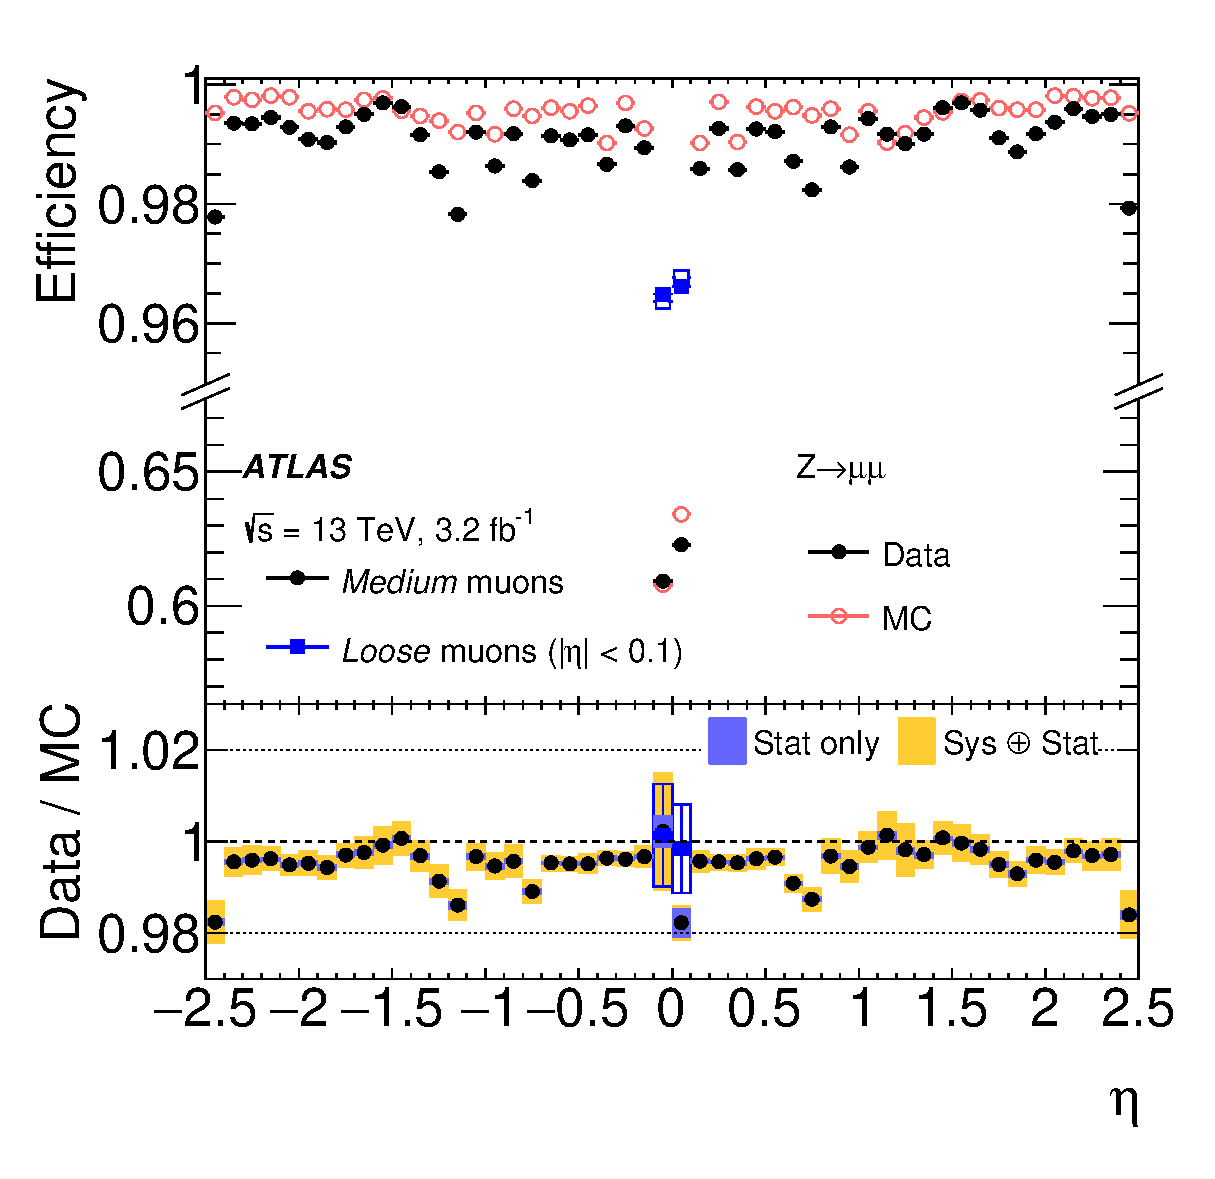
\includegraphics[width=0.55\textwidth]{figures/MuonReco/MuonEff.eps}\hspace{0.05\textwidth}
\end{center}
\caption{Muon reconstruction efficiency for loose and medium muons.\cite{MuonReco}  Loose and medium muons are identical except in the $|\eta| < 0.1$ region where loose muons also accept calo-tagged and segment tagged muons to recover efficiency.}
\label{fig:muoneff} 
\end{figure}

\indent Muon momentum is calibrated to $J/\psi\rightarrow \mu\mu$ or $Z\rightarrow\mu\mu$ events in data.  The $\pT$ of individual tracks are corrected to account for any inaccuracies in the detector description such as the magnetic field, dimensions of the detector and the amount of energy loss in the calorimeters.  Correction parameters are extracted using a likelihood fit to data with templates derived from MC. MS/ID alignment is also studied using special runs with no magnetic field. The correction parameters differ for different sections of $\eta$ and $\phi$ regions because of the different amount of magnetic fields and independent alignment performed in each section. \\

\indent On top of the total correction to the central value of the $\pt$, the momenta resolution is also estimated using data.  The MC is smeared such that the reconstructed di-muon mass peak agrees between data and MC.  The muon momenta resolution is described according to equation \ref{eqn:muonReso}\\

\begin{equation}
\frac{\sigma(\pt)}{\pt} = r_0/\pt~\oplus~r_1~\oplus~r2~\dot~\pt
\label{eqn:muonReso}
\end{equation}

\indent $r_0/\pt$ accounts for fluctuations in the energy loss in the calorimeter material.  $r_1$ describes multiple scattering, local disturbances in the magnetic field and displacement of hits.  $r2~\dot~\pt$ describes the spacial resolution on the detector hits and any potential mis-alignment in the MS.  Uncertainty with all 3 parameters $r_0$, $r_1$ and $r_2$ are all extracted using a likelihood fit to $J/\psi\rightarrow \mu\mu$ or $Z\rightarrow\mu\mu$ events in data. \\

The affect of muon momenta calibration on the MC description of $J/\psi\rightarrow \mu\mu$ and $Z\rightarrow\mu\mu$ mass peaks can be seen in figure \ref{fig:muonCalib}. \\

\begin{figure}[htb]
  \begin{center}
    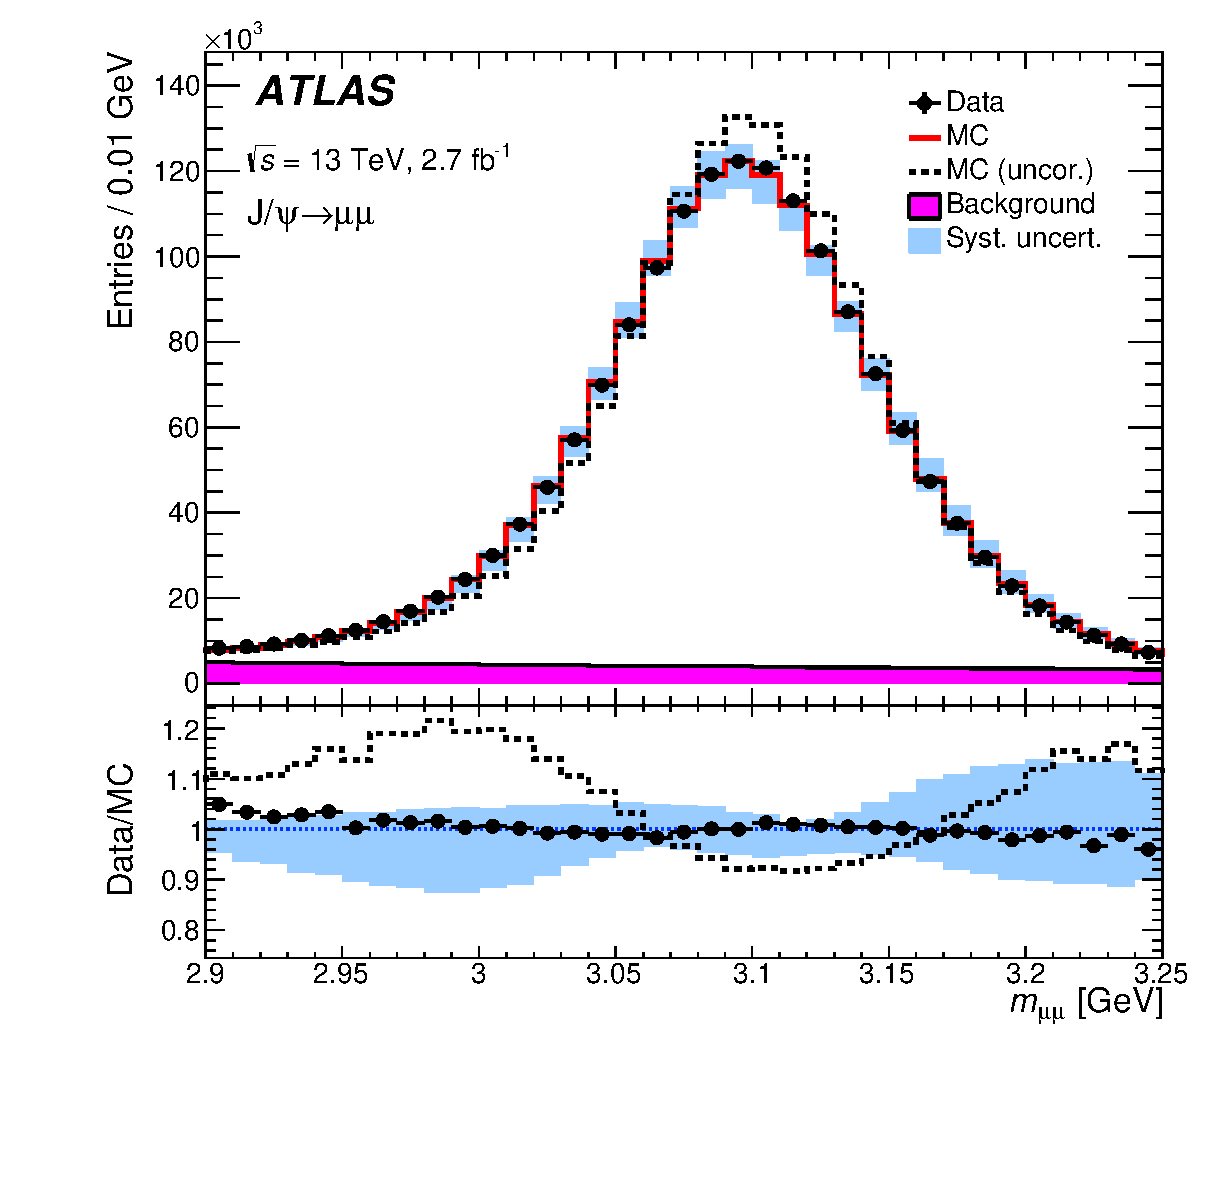
\includegraphics[width=0.45\textwidth]{figures/MuonReco/JPsiMass.eps}\hspace{0.05\textwidth}
    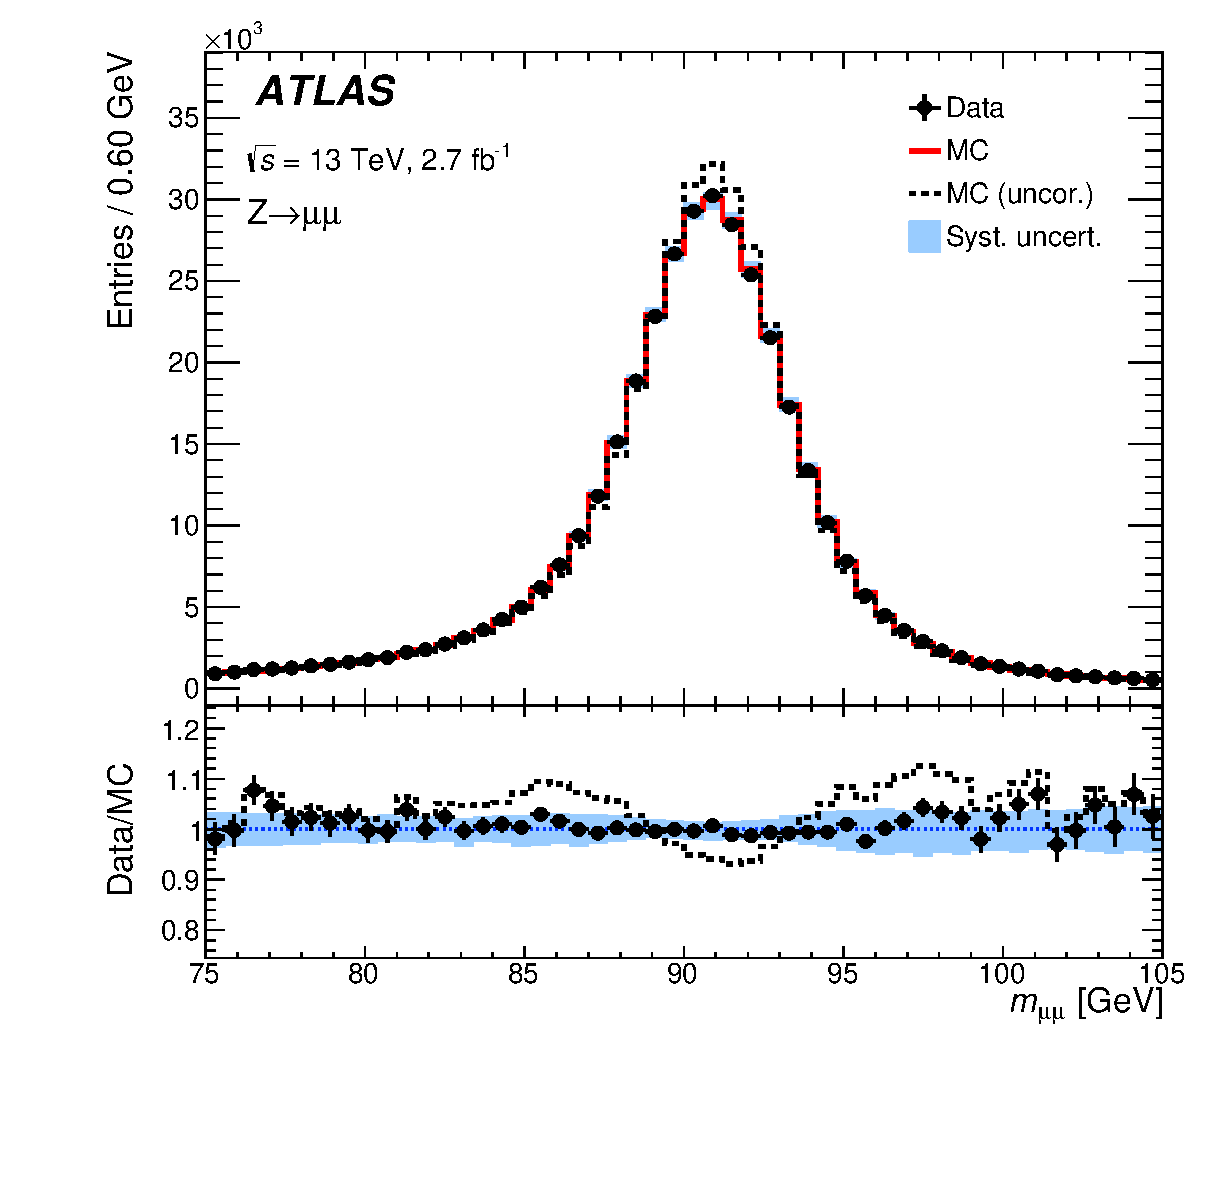
\includegraphics[width=0.45\textwidth]{figures/MuonReco/ZMass.eps}\hspace{0.05\textwidth}
\end{center}
\caption{Dimuon invariant mass before and after muon momenta calibration in data and MC.\cite{MuonReco}}
\label{fig:muonCalib} 
\end{figure}

\section{Missing Transverse Momentum}
\label{sec:reco:MET}

\indent Stable or metastable particles which only interact via the weak force and gravity cannot be directly detected at ATLAS.  In SM, these particles correspond to neutrinos.  In BSM models, there maybe many other weakly interacting particles including WIMPs, gravitons, and a stable neutral SUSY LSP. \\

\indent The presence of weakly interacting particles is inferred through conservation of transverse momentum.  The total transverse momentum is zero in the initial colliding partons at the LHC.  Therefore, any momentum imbalance in the transverse plane must be due to undetected particles in the final state.  \\

\subsection{$\met$ Reconstruction}
\label{sec:MET:reco}

\indent We reconstruct the $\met$ according to equation \ref{eqn:metReco}.  The first term is a negative vector sum of all hard fully calibrated objects and the second term represents the $\vec{E}_t$ of all soft objects in the interaction.  \\

\begin{equation}
\met = - ( \sum_{hard~objects} E_T + \sum_{soft} E_T ) 
\label{eqn:metReco}
\end{equation}

\indent Fully calibrated hard objects include muons, electrons, photons and jets that satisfy their respective {\tt Baseline} selections.  {\tt Baseline} selections applies a loose set of $\pt$ and quality requirements to ensure well reconstructed objects.  {\tt Baseline} object definitions can be found in chapter \ref{chap:objects}. \\

\indent Hadronic taus are not independently reconstructed and calibrated.  Therefore, hadronic taus will most likely be reconstructed as hadronic jets for our analysis.  An overlap removal algorithm have been applied to the {\tt Baseline} objects to remove any potential duplicate objects. \\

\indent We use a track based method called Track Soft Term (TST) \cite{METReco} to reconstruct the contribution from soft objects.  TST build the $\met$ that is not associated with any hard objects by summing the $\pt$ of ID tracks. \\

\indent TST has the advantage of being relatively robust against pileup interactions because TST use ID tracks that are matched with the primary vertex. However TST cannot measure the contribution to $E_T$ from neutral particles because neutral particles do not leave tracks in the ID.  TST is the standard method of estimating $\met$ at ATLAS in Run 2 due to the high pileup conditions. \\

\indent  Only tracks with $\pt > 400 \mev$ are accepted and a number of track quality requirements are applied.  The track quality requirement follows recommendations from the ATLAS tracking performance group and include a minimum of $7$ silicon hits and a requirement on the track $d_0$.  Any tracks within a $\Delta R$ of 0.05 of any electron or photon cluster, the ID tracks of muons, and any ID tracks matched to jets are removed to avoid double counting.  Further details on TST can be found in \cite{METReco}.  \\

\indent $\met$ reconstructed using this method is the standard $\met$ used throughout all signal, control and validation regions in this analysis and is simply referred to as $\met$.  This method of reconstructing $\met$ is also referred to as TST $\met$ to distinguish it from an alternative method of reconstructed $\met$ called track $\met$ described in section \ref{sec:reco:trkMET}. \\

\subsection{Track $\met$ Reconstruction}
\label{sec:reco:trkMET}

\indent Track $\met$ ($\mettrk$) forms a complementary method of reconstructing missing transverse energy.  $\mettrk$, defined in equation \ref{eqn:mettrkReco}, is reconstructed using a negative vector sum of all accepted ID tracks.  \\

\begin{equation}
\mettrk = - \sum_{ID tracks} \pt  
\label{eqn:mettrkReco}
\end{equation}

\indent ID tracks must pass the same requirements described in section \ref{sec:MET:reco} for the TST but no attempt is made at removing tracks that are associated with hard objects.  The one exception to this is tracks associated with an electron.  Because of the high number of interaction expected between an electron and the material in the ID, electron tracks are replaced with the electron calorimeter cluster instead.  \\

\indent Track $\met$ is very robust against pileup conditions ATLAS has very good vertex resolution but neglects the presence of neutral particles.  Track $\met$ is also limited by $\eta$ coverage of the ID which only extends to an $|\eta| < 2.5$.  We use track $\met$ as a cross check on the object based $\met$ reconstruction described in \ref{sec:MET:reco}. Both object based and track based $\met$ must agree loosely in direction for our analysis.  \\

\subsection{$\met$ Performance}
\label{sec:reco:METPerform}

\indent $\met$ performance maybe measured using a number of processes include $Z\rightarrow ll$, $W\rightarrow l\nu$ and ttbar.  $Z\rightarrow ll$ produced with additional jets is considered the gold standard.  Very little intrinsic $\met$ is produced in the $Z\rightarrow ll$ plus jets process.  This presents a good opportunity to study the effect of the $\met$ soft term calculation since no hard invisible particles exist.  The only variable intrinsic to $\met$ reconstruction is the soft term.  All other terms in $\met$ reconstruction depend directly on the resolution of the respective reconstructed hard objects.  $W\rightarrow l\nu$ is also used to study a topology with a high-$\pt$ neutrino and therefore intrinsic $\met$ and ttbar is used to study topologies with a large number of jets. \\

\indent Results from $Z\rightarrow ll$ performance study \cite{METReco} will be summarized here.  The $W\rightarrow l\nu$ $\met$ and ttbar study will not be covered here but further detail can be found in \cite{METReco}. \\

\indent $Z\rightarrow \mu\mu$ events are selected by requiring exactly two same flavor, opposite signed muons with $\pt > 25 \gev$. The dilepton invariant mass must be within $25 \gev$ of the $Z$ mass. \\
%\indent $W\rightarrow e\nu$ events are selected by requiring exactly one electron in the event.  The electron must have $\pt > 17 \gev$.  The TST $\met$ must be greater then $25 \gev$ and the reconstructed transverse mass must be consistent with a $W$ boson decay at greater then $50 \gev$.\\

\indent Distribution of the $\met$ resolution in $Z\rightarrow \mu\mu$ events , defined as the root-mean-squared (RMS) of the $\met$ distribution is shown in figure \ref{fig:MET_reso}.  The $\met$ resolution degrades both with the total amount of $E_T$ in the event and the number of reconstructed vertexes.\\

\begin{figure}[htb]
  \begin{center}
    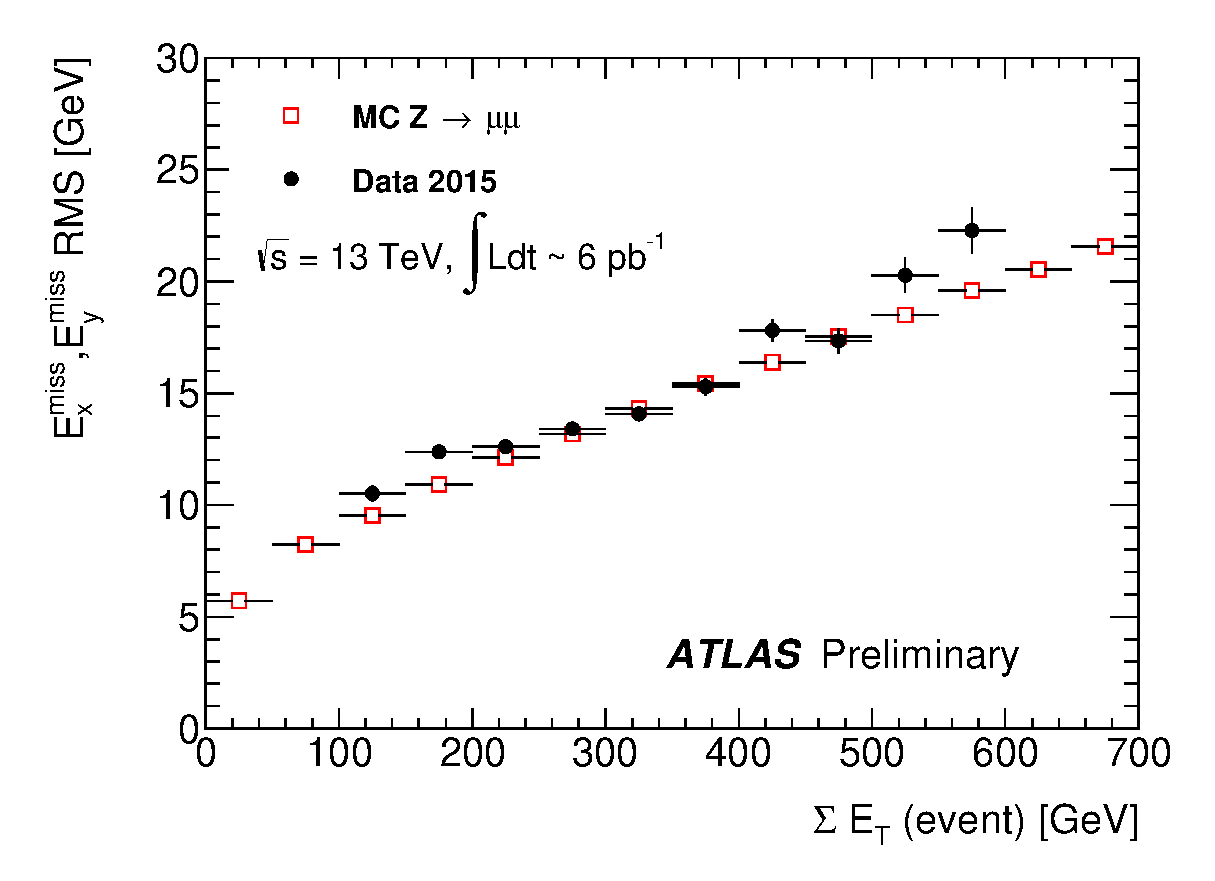
\includegraphics[width=0.45\textwidth]{figures/METCalib/METReso_Et.eps}\hspace{0.05\textwidth}
    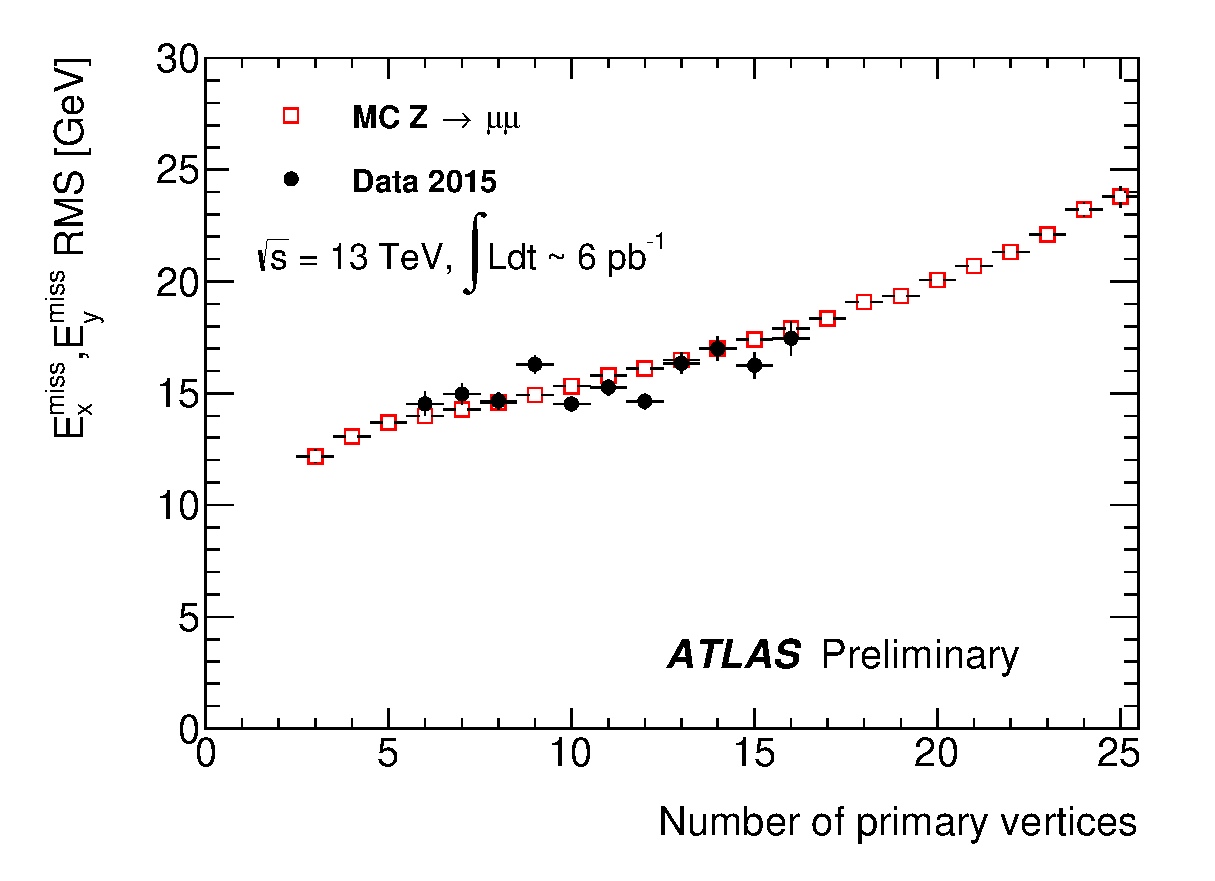
\includegraphics[width=0.45\textwidth]{figures/METCalib/METReso_nVtx.eps}\hspace{0.05\textwidth}
\end{center}
\caption{Distribution of the TST $\met$ resolution relative to the total $E_t$ of reconstructed objects in $Z\rightarrow \mu\mu$ events and Distribution of the TST $\met$ resolution relative to the number of reconstructed vertexes in $Z\rightarrow \mu\mu$ events.  $\met$ resolution degrades as $E_T$ and pileup increases.  (Figures taken from \cite{METReco})}
\label{fig:MET_reso} 
\end{figure}

%\indent Biases in the reconstructed $\met$ can be both in the form of direction.  The mean value of the reconstructed $\met$ projected onto the direction of flight of the $Z$ boson in the transverse plane ($A_Z$) is a useful quantity to describe any bias in the $\met$ soft term.  $Because the $Z\rightarrow \mu\mu$ do not contain true $\met$, an unbiased $\met$ would have an average of zero in the projection of the $\met$ onto the $Z$ direction.  \\

%\indent Distributions showing the bias on the reconstructed $\met$ in direction is shown in figure \ref{}.




